\section{Законы Ньютона для материальной точки и твёрдого тела. Законы сохранения энергии, импульса, момента импульса.}

\textbf{Динамика} - изучение движения материальных тел под действием приложенных к ним систем сил с учётом инертности самих тел. Вводят абстрактное понятие о материальной точке, как о точке обладающей массой. Материальная точка - модель простейшего материального объекта, обладающего массой и размерами, формой, вращением и структурой которого можно пренебречь.

Для описания реального твердого тела используют модель абсолютно твердого тела, т.е. совокупности материальных точек, расстояния между которыми постоянны. Движение в общем случае складывается из вращательного и поступательного. Материальное тело можно рассматривать, как материальную точку в тех случаях, когда можно не принимать во внимание вращательную часть движения тела.

\textbf{Первый закон Ньютона (Закон инерщии):}
Изолированная от внешних воздействий материальная точка сохраняет своё состояние покоя (равномерного прямолинейного движения) пока приложенные силы не заставят её изменить это состояние относительно инерциальных систем отсчёта.

%Для твёрдого тела: Если на тело не действуют другие тела (силы), то оно сохраняет состояние покоя или равномерного прямолинейного движения.

\textbf{Второй закон Ньютона (основной закон динамики):}
Произведение массы материальной точки на ускорение, которое она получает под действием данной силы равно по модулю этой силы, а направление ускорения совпадает с направлением силы в инерциальной системе отсчета:

$$
\vec{F}=m \vec{a}
$$

То есть при действии на точку одной и той же силы точка с большей массой приобретёт меньшее по величине ускорение (масса является мерой инертности материальной точки).

Если на точку действует несколько сил, то: $\sum \vec{F}=m \vec{a}$

Для твёрдого тела: Твердое тело, в отличие от материальной точки, может обладать поступательным и вращательным движением, в связи с чем основной закон динамики для него примет вид:

\begin{enumerate}
  \item $\sum_{k}^{\text {внешн }} \vec{F}=M \vec{a}_{c}$ (для поступательного движения), где $\Sigma F$ - векторная сумма внешних сил, $\overline{a_{c}}$ - ускорение центра масс системы

  \item $\sum M_{z}=J_{z \varepsilon}$ (для вращательного вращения относительно некоторой оси z), где $\sum M_{z}-$ сумма вращающих моментов сил, $J_{z}$ - момент инерции относительно оси z, $\varepsilon$ - угловое ускорение. Это аналог второго закона Ньютона для вращательного движения, из которого следует, что угловое ускорение $\bar{\varepsilon}$ твердого тела при вращении вокруг неподвижной оси прямо пропорционально вращающему моменту и обратно пропорционально моменту инерции относительно этой оси.

\end{enumerate}

\textbf{Третий закон Ньютона (закон равенства действия и противодействия):}
Две материальные точки действуют друг на друга с силами: 1) равными по модулю; 2) направленными вдоль прямой, соединяющей эти точки, в противоположные стороны. Силы не образуют равновесия, поскольку они приложены к разным точкам.

Для твёрдого тела: при взаимодействии тел сила действия со стороны одного тела на другое равна по величине и противоположна по направлению силе, действующей со стороны другого тела на первое.

Принцип независимости действия сил: Каждая сила, приложенная к материальной точке, сообщает ей одно и то же ускорение, независимо от того действует она одна или в совокупности с другими силами. Закон сохранения энергии: При движении механической системы в потенциальном силовом поле её полная механическая энергия сохраняется. $\mathrm{T}_{1}+\Pi_{1}=\mathrm{T}_{2}+\Pi_{2}=$ const, где $\mathrm{T}-$ кинетическая энергия, $\Pi-$ потенциальная. Для механической систему кинетическая энергия равна арифметической сумме кинетических энергий всех точек механической системы.

\textbf{Закон сохранения импульса:} Импульс (количество движения) точки - векторная динамическая характеристика её движения. Равна произведению массы точки на вектор её скорости $(\bar{p}=m \bar{v})$. Импульс системы материальных точек - геометрическая сумма всех ее импульсов:

$$
\vec{p}=\sum_{k=1}^{n} m_{k} \overrightarrow{v_{k}}
$$

Тогда изменение импульса:

$$
\frac{d \vec{p}}{d t}=\sum_{k=1}^{n} m_{k} \vec{a_{k}}=\sum_{k=1}^{n} \Vec{F_{k}}^{\text{внешн}}+\sum_{k=1}^{n} \vec{F_{k}}^{\text{внутр}}
$$

Учитывая, что сумма всех внутренних сил $0: \sum_{k=1}^{n} \vec{F_{k}}^{\text{внутр}}=0$, то:

$$
\frac{d \vec{p}}{d t}=\sum_{k=1}^{n} \Vec{F_{k}}^{\text{внешн}}
$$

Если система замкнута, то внешние силы на нее не действуют, поэтому изменение импульса будет 0.

\textbf{Закон сохранения импульса.} 

В замкнутой системе векторная сумма импульсов тел не меняется при любых движениях и взаимодействиях между телами системы.

Закон сохранения момента импульса: если сумма моментов относительно данного центра всех приложенных к системе внешних сил равна нулю, то главный момент количеств движения системы относительно этого центра будет количественно и по направлению постоянен.


Моментом импульса материальной точки А относительно неподвижной (произвольной) точки О называется физическая величина, определяемая векторным произведением $\vec{L}=[\bar{r} \bar{p}]$, где $\bar{r}-$ радиусвектор, проведенный из точки $\mathrm{O}$ в точку $\mathrm{A}, \quad \bar{p}=m \bar{V}$ - импульс материальной точки. Модуль вектора момента импульса $\mathrm{L}=\mathrm{r} \mathrm{p} \sin \alpha=\mathrm{m} \mathrm{~V}\mathrm{r} \sin \alpha=\mathrm{p}  \mathrm{d}$, где $\alpha$ - угол между векторами $\bar{r}$ и $\bar{p}, \mathrm{~d}$ - плечо вектора $\bar{p}$ относительно точки $\mathrm{O}$ :

\begin{figure}[h!]
    \centering
    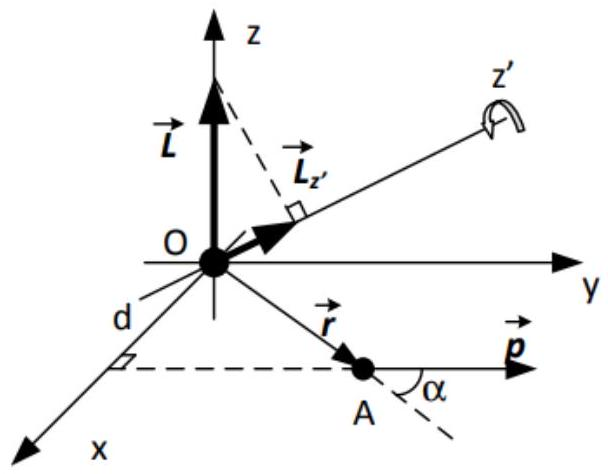
\includegraphics[width=0.5\textwidth]{2023_05_21_6e9b4e8657e82b213c6ag-03}
\end{figure}

Моментом импульса относительно оси z называется величина $\mathrm{L}_{\mathrm{z}}$, равная проекции на эту ось вектора момента импульса $\vec{L}$, определенного относительно произвольной точки O данной оси z. Значение момента импульса $\mathrm{L}_{\mathrm{z}}$ не зависит от положения точки $\mathrm{O}$ на оси z. При непрерывном распределении массы момент импульса относительно оси z равен:

$$
\overrightarrow{L_{z}}=J_{z} \overrightarrow{\omega_{z}}
$$

где $J_{z}$ - момент инерции тела относительно оси z, $\omega_{z}$ - угловая скорость вращения.

Момент импульса материальной точки или твердого тела связан с моментом приложенных сил следующим соотношением, называемым уравнением моментов:

$$
\frac{d \vec{L}}{d t}=\vec{M}
$$

Из уравнения моментов следует, что, если результирующий момент сил, действующий на систему материальных точек или твердое тело равен нулю (замкнутая система), то момент импульса такой системы остается постоянным:

$$
\vec{L}=\text { const }
$$

Если тело вращается вокруг закрепленной оси z, то сохраняется проекция момента импульса тела на эту ось:

$$
\overrightarrow{L_{z}}=\text { const }
$$

 \section{Теоремы об изменении количества движения материальной системы; об изменении главного момента количества движения материальной системы; об изменении кинетической энергии материальной системы.}


\begin{figure}[h!]
    \centering
    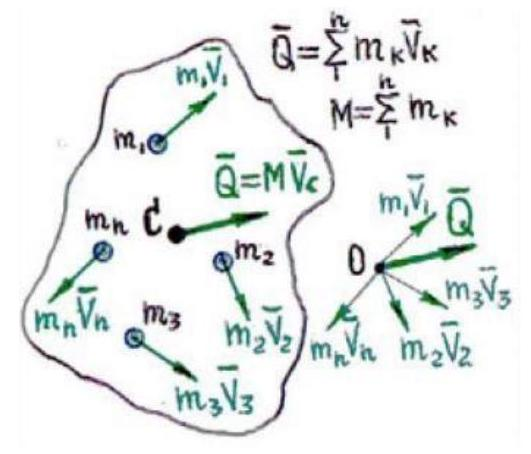
\includegraphics[width=0.5\textwidth]{2023_05_21_6e9b4e8657e82b213c6ag-05}
\end{figure}


\textbf{Теорема об изменении количества движения материальной системы:} Количество движения $\mathrm{mV}$ точки - произведение массы точки на вектор её скорости. Количеством движения системы - геометрическая сумма количеств движения всех её точек:

$$
\vec{Q}=\sum_{k=1}^{n} m_{k} \overrightarrow{v_{k}}
$$

Учитывая теорему о движении центра масс:

$$
M \vec{V}_{c}=\sum_{k=1}^{n} m_{k} \overrightarrow{v_{k}}
$$

Получаем, что:

$$
\vec{Q}=M \vec{V}_{c}
$$

Рассмотрим систему из $n$ материальных точек. Составим для этой системы дифференциальные уравнения движения и сложим их почленно:

$$
\frac{d \vec{Q}}{d t}=\frac{d}{d t} \sum_{k=1}^{n} m_{k} \overrightarrow{v_{k}}=\sum_{k=1}^{n} m_{k} \overrightarrow{a_{k}}=\sum_{k=1}^{n} \vec{F_{k}}^{\text{внутр}}+\sum_{k=1}^{n} \vec{F_{k}}^{\text{внешн}}
$$

С учетом того, что сумма внутренних сил 0 (3 закон Ньютона), то:

$$
\frac{d \vec{Q}}{d t}=\sum_{k=1}^{n} \\Vec{F_{k}}^{\text{внешн}}
$$

Тогда \textbf{теорема об изменении количества движения материальной системы:}

\begin{enumerate}
  \item В дифференциальной форме: производная по времени от количества движения системы равна геометрической сумме всех действующих на систему внешних сил.

  \item В интегральной форме: изменение количества движения системы за некоторый промежуток времени равно сумме импульсов, действующих на систему внешних сил за тот же промежуток времен.

\end{enumerate}

\textbf{Теорема об изменении главного момента количества движения материальной системы:}

Главный момент количества движения (кинетический момент) системы относительно данного центра $\mathrm{O}$ - величина $\mathrm{K}_{\mathrm{O}}$, равная геометрической сумме моментов количеств движения всех точек системы относительно этого центра:

$$
\overrightarrow{K_{O}}=\sum_{k=1}^{n} \overrightarrow{M_{0}}\left(m_{k} \overrightarrow{v_{k}}\right)=\sum_{k=1}^{n}\left[\overrightarrow{r_{k}} \times\left(m_{k} \overrightarrow{v_{k}}\right)\right]
$$

Рассмотрим одну материальную точку системы. Производная моментов количества движения равна (аддитивность сил и моментов):

$$
\frac{d}{d t} \overrightarrow{M_{0}}\left(m_{k} \overrightarrow{v_{k}}\right)=\overrightarrow{M_{0}}\left(\Vec{F_{k}}^{\text{внешн}}\right)+\overrightarrow{M_{0}}\left(\vec{F_{k}}^{\text{внутр}}\right)
$$

Где силы - равнодействующие внутренние и внешние составляющие, действующие на данную точку.

Тогда составляя данные уравнения для всех точек системы и складывая их почленно, получаем:

$$
\frac{d}{d t} \sum \overrightarrow{M_{0}}\left(m_{k} \overrightarrow{v_{k}}\right)=\sum \overrightarrow{M_{0}}\left(\Vec{F_{k}}^{\text{внешн}}\right)+\sum \overrightarrow{M_{0}}\left(\vec{F_{k}}^{\text{внутр}}\right)
$$

Но последняя сумма равно 0 (так как по 3 закону Ньютона сумма всех внутренних сил скомпенсируется, как и сумма моментов этих сил). Тогда:

$$
\frac{d \overrightarrow{\mathrm{K}_{\mathrm{o}}}}{d t}=\sum \overrightarrow{M_{0}}\left(\Vec{F_{k}}^{\text{внешн}}\right)
$$

Формулировка теоремы: производная по времени от главного момента количества движания системы относительно некоторого неподвижного центра равна сумме моментов всех внешних сил системы относительно того же центра.

$$
\vec{F}=m \frac{d \vec{v}}{d t}
$$

\textbf{Теорема об изменении кинетической энергии:}


1) Для материальной точки:


\begin{figure}[h!]
    \centering
    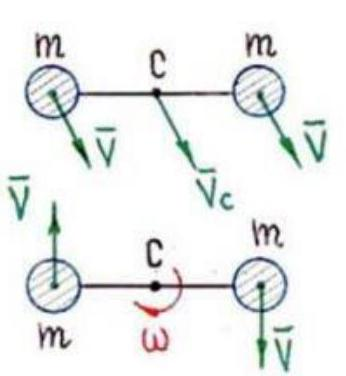
\includegraphics[width=0.4\textwidth]{2023_05_21_6e9b4e8657e82b213c6ag-06}
\end{figure}
Кинетическая энергия материальной точки - скалярная характеристика ее движения

$\mathrm{T}=\left(mv^{2} / 2\right)$.

В простейшей системе из двух равных по массе точек с поступательным движением $v$. Тогда очевидно, что

$$
T=\frac{m v^{2}}{2}+\frac{m v^{2}}{2}=m v^{2}
$$

Если вращательное движение с постоянной угловой скоростью $\omega$, то точки будут иметь одинаковые по величине скорости: $\mathrm{V}=\omega r$, тогда суммарная кинетическая энергия:

$$
T=\frac{m V^{2}}{2}+\frac{m V^{2}}{2}=m V^{2}
$$

То есть система обладает одинаковыми кинетическими энергиями, хотя движения разные. Кинетическая энергия не учитывает направленность движения.

Из второго закона Ньютона силу можно выразить как:

$$
\vec{F}=m \frac{d \vec{v}}{d t}
$$

Умножая скалярная данное произведение на dr получаем:

$$
\vec{F} d r=m \frac{d \vec{v}}{d t} d r=m \frac{d r}{d t} d \vec{v}=m v d \vec{v}=d\left(\frac{m v^{2}}{2}\right)=d A
$$

Это - математическая трактовка теоремы об элементарном изменении кинетической энергии точки: элементарное изменение кинетической энергии точки равно элементарной работе действующей на точку силы.

2)Для материальной системы:


Кинетической энергия системы называют скалярную величину $\mathrm{T}$, равную сумме кинетических энергий всех точек системы:

$$
T=\sum \frac{m v^{2}}{2}
$$

Доказанную выше теорему об элементарной изменении кинетической энергии точки применяем для всех точек системы и складываем почленно, получаем:

$$
d \sum\left(\frac{m v^{2}}{2}\right)=d T=\sum d A^{\text {внешних }}+\sum d A^{\text {внутренних }}
$$

Проинтегрировав обе части получаем:

$$
T_{1}-T_{0}=\sum A^{\text {внешних }}+\sum A^{\text {внутренних }}
$$

Это математическое представление теоремы об изменении кинетической энергии механической системы: изменение кинетической энергии системы на некотором её перемещении равно сумме работ всех внешних и внутренних сил, действующих на систему на этом перемещении.

\section{Относительное движение. Сложное движение. Силы инерции. Связи - идеальные, голономные, неголономные.}

Движение точки, рассматриваемое одновременно в неподвижной и подвижной систем отсчёта, называют сложным. При этом движение точки относительно неподвижной системы отсчёта называется абсолютным. Движение точки относительно подвижной системы отсчёта - относительное. Движение подвижной системы отсчета относительно неподвижной - переносное.



\begin{figure}[h!]
    \centering
    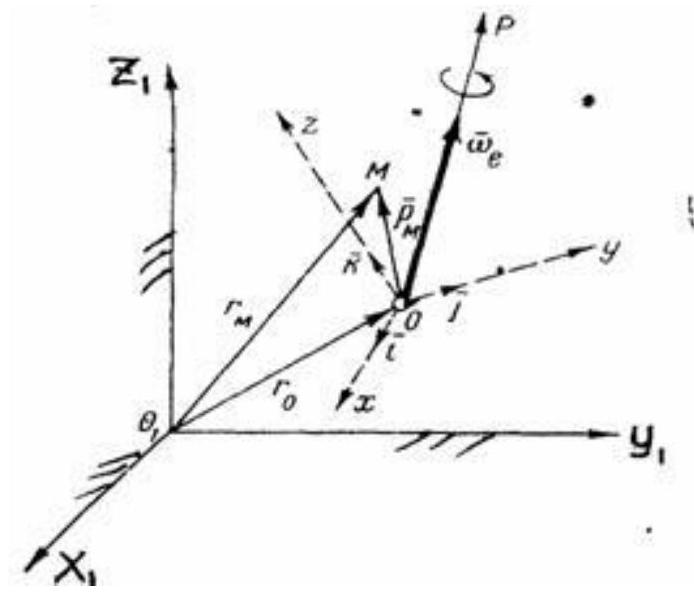
\includegraphics[width=0.5\textwidth]{2023_05_21_6e9b4e8657e82b213c6ag-07}
\end{figure}


$\mathrm{O}_{1} \mathrm{X}_{1} \mathrm{Y}_{1} \mathrm{Z}_{1}-$ неподвижная система координат. Вводится подвижная система координат OXYZ, совершающая заданное движение относительно неподвижной. Движение т.М относительно подвижной системы координат называется относительным. Траектории т.М относительно подвижной системы координат называется относительной. Скорость ОXYZ относительно $\mathrm{O}_{1} \mathrm{X}_{1} \mathrm{Y}_{1} \mathrm{Z}_{1}$ называется переменной. Скорость т.М относительно $\mathrm{O}_{1} \mathrm{X}_{1} \mathrm{Y}_{1} \mathrm{Z}_{1}$ называется абсолютной.

\textbf{Tеорема о сложении скоростей:} Вектор абсолютной скорости точки при сложном движении равен геометрической сумме её переносной и относительно скоростей:

$$
\bar{v}_{\text {абс }}=\bar{v}_{\text {пер }}+\bar{v}_{\text {отн }}
$$

\textbf{Теорема о сложении ускорений (Теорема Кориолиса):}


$$
\overrightarrow{\mathrm{a}_{\mathrm{aбc}}}=\overrightarrow{\mathrm{a}_{\text {отн }}}+\overrightarrow{\mathrm{a}_{\text {перен }}}+2 \overrightarrow{\boldsymbol{\omega}_{\text {перен }}} \times \overrightarrow{\boldsymbol{v}_{\text {отн }}}, \quad
\text{где } \overrightarrow{\mathrm{a}_{\text {кориолисово }}}=\mathbf{2} \overrightarrow{\boldsymbol{\omega}_{\text {перен }}} \times \overrightarrow{\boldsymbol{v}_{\text {отн }}}
$$


\begin{figure}[h!]
    \centering
    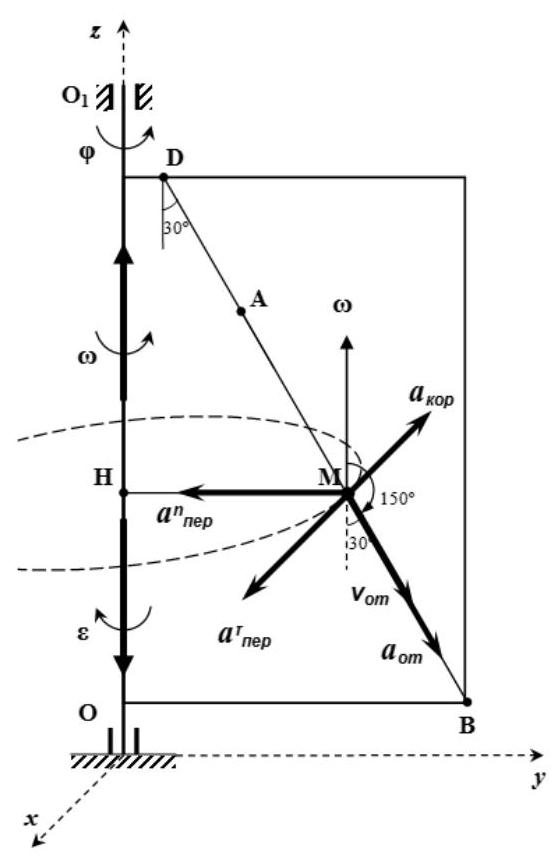
\includegraphics[width=0.5\textwidth]{2023_05_21_6e9b4e8657e82b213c6ag-08(1)}
\end{figure}


Кориолисово ускорение характеризует:

\begin{enumerate}
  \item Изменение модуля и направления переносной скорости точки из-за её относительности движения

  \item Изменение направления относительной скорости из- за вращательного переносного движения
\end{enumerate}

Направление кориолисова ускорения определяется по правилу Жуковского: 
Вектор относительной скорости спроецировать на плоскость, перпендикулярную переносной угловой скорости, и повернуть проекцию на $90^{\circ}$ в сторону вращения.

\textbf{Силы инерџии}


В общем случае сила инерции -векторная величина, равная произведению массы материальной точки на ее ускорение и направленная противоположно ускорению. Пусть F- активные силы, a R- силы реакции, тогда по второму закону Ньютона:

$$
m \overrightarrow{\mathrm{a}_{\mathrm{a} c}}=\sum \vec{F}+\vec{R}
$$

Раскрывая абсолютное ускорение по теореме Кориолиса:

$$
\begin{gathered}
m\left(\overrightarrow{\mathrm{a}_{\mathrm{oтн}}}+\overrightarrow{\mathrm{a}_{\text {перен }}}+\overrightarrow{\mathrm{a}_{\text {кориолиса }}}=\sum \vec{F}+\vec{R}\right. \\
m \overrightarrow{\mathrm{a}_{\mathrm{oтн}}}=\sum \vec{F}+\vec{R}-m \overrightarrow{\mathrm{a}_{\text {перен }}}-m \overrightarrow{\mathrm{a}_{\text {кориолиса }}} \\
m \overrightarrow{\mathrm{a}_{\mathrm{oтн}}}=\sum \vec{F}+\vec{R}+\overrightarrow{F_{\text {перен }}}+\overrightarrow{F_{\text {кориолиса }}}
\end{gathered}
$$
Тогда $\overrightarrow{F_{\text {перен }}=}-m \overrightarrow{\mathrm{a}_{\text {перен }}}-$ переносная сила инерции, 


$\overrightarrow{F_{\text {кориолиса }}}=-m \overrightarrow{\mathrm{a}_{\text {кориолиса) }}} $ кориолисова сила инерции.


\textbf{Связи}


Если на движение тела наложены некоторые ограничения, то говорят, что на движение тела нажжены связи. Связи - тела, ограничивающие свободу перемещения данной точки или тела, наложенным на данную точку или тело.

Идеальные связи: в которых отсутствует трение. При этом сумма элементарных работ реакций связей на элементарных перемещениях равна нулю.

Основные виды идеальных связей:

\begin{figure}[h!]
    \centering
    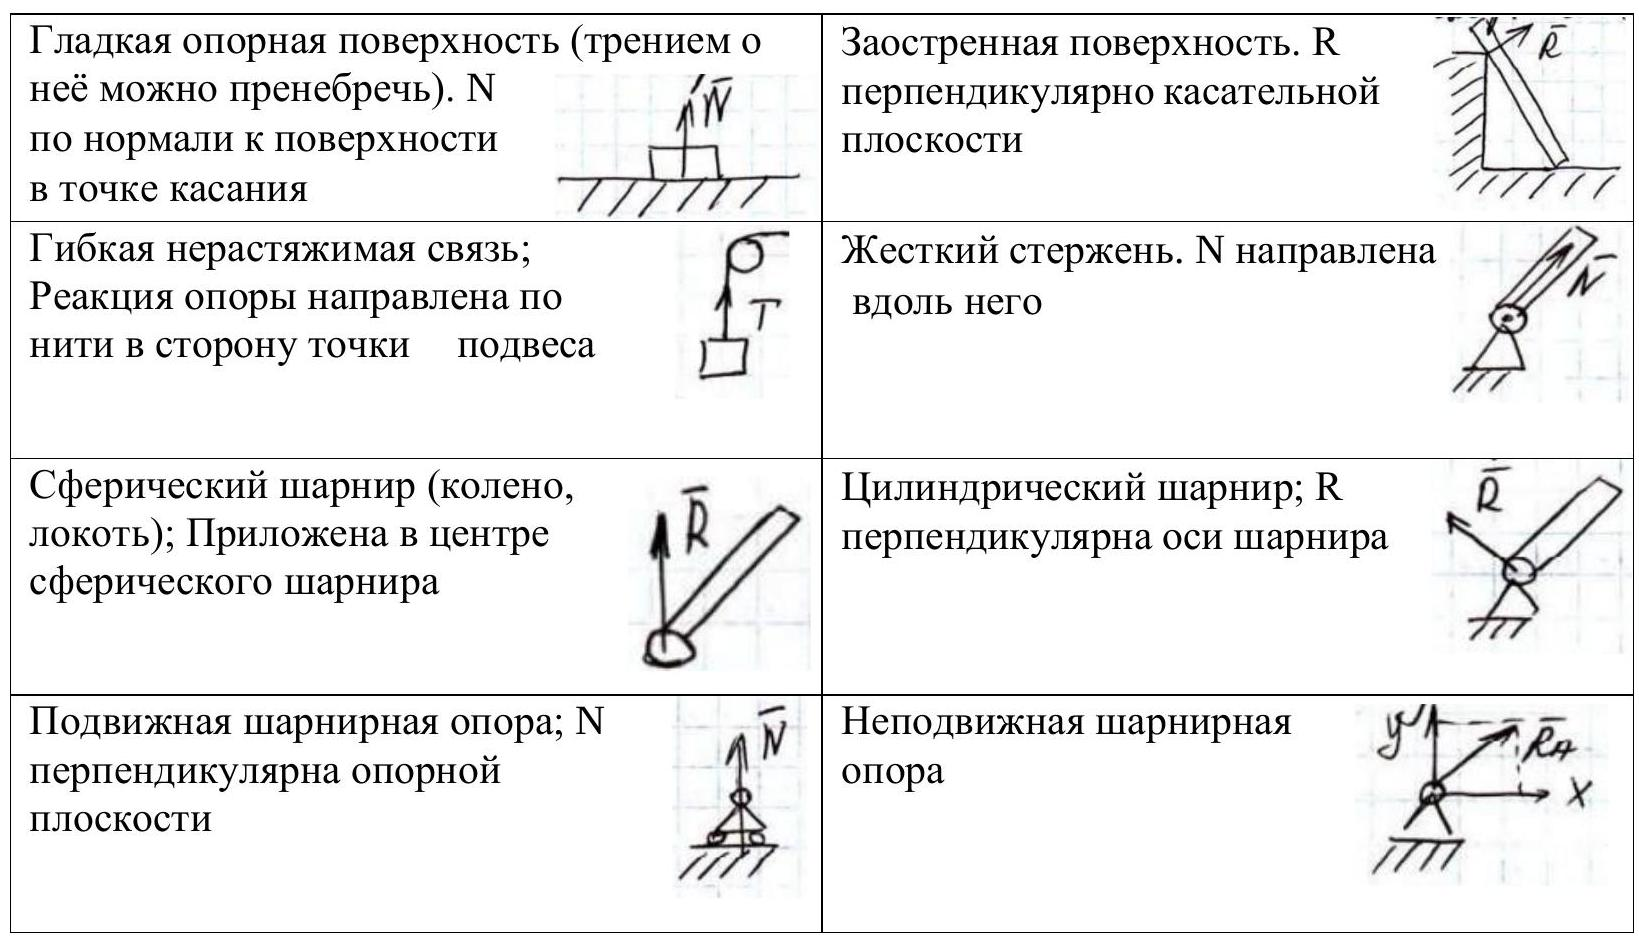
\includegraphics[width=1\textwidth]{2023_05_21_6e9b4e8657e82b213c6ag-09}
\end{figure}


Связи, налагающие ограничения на положения точек системы - геометрические, а налагающие ограничения еще и на скорости- кинематические (дифференциальньими). Геометрические и интегрируемые дифференциальные связи называют связями голономными, а неинтегрируемые дифференциальные связи - неголономными. По виду связей механические системы тоже разделяют на голономные (с голономными связями) и неголономныlе (содержащие неголономные связи).

\section{Уравнения Лагранжа второго рода.}
Общее уравнение динамики:
Рассмотрим систему материальных точек, на которую наложены стационарные, идеальные, голономные связи. Тогда \textbf{принцип возможных перемещений}: При равновесии материальной системы с идеальными и стационарными связями сумма работ всех активных, задаваемых, сил на любом возможном перемещении системы из положения равновесия равна нулю:

$$
\sum_{k=1}^{n} \overrightarrow{F_{k}^{\text{акт}}} \delta \overrightarrow{r_{k}}=\sum_{k=1}^{n} \delta A_{k}^{\text{акт}}=0
$$

Принцип Даламбера позволяетрассматривать динамическую систему как статическую, если к ней добавить силы инерции:

$$
\sum_{k=1}^{n} \delta A_{k}^{\text {акт }}+\sum_{k=1}^{n} \delta A_{k}^{\text {инерц }}=0
$$
Это общее уравнение динамики.


\textbf{Обобщенные координаты:} Положение механической системы, состоящей из $\mathrm{n}$ материальных точек определяется $3 \mathrm{n}$ декартовыми координатами: $x_1, y_1, x_1, ..., x_n, y_n, z_n.$. Пусть на систему наложено $l$ геометрических удерживающих связей. Связи накладывают ограничения на декартовы координаты, записываемые в виде соотношений: $f k(x_1, y_1, z_1, \ldots$, $x_n, y_n, z_n)=0$ гдe $k=1 \ldots l$ - уравнения связей. Из уравнения связей определяют $Зn-l=s$ координат, все декартовы координаты однозначно выражают через $s$ каких-либо независимых параметров $q_1, q_2, \ldots, q_s$, которые называются обобщенными координатами. 

Обобщенные координаты - любые независимые параметры, которые полностью и однозначно определяют положение системы. Тогда в обобщенных координатах общее уравнение динамики может быть записано через частные производные:

Где $\mathrm{Q}_{\mathrm{i}}$ - обобщенные силы:

$$
\sum_{i=1}^{s}\left(Q_{i}^{\text {акт }}+Q_{i}^{\text {инерц }}\right) \delta q_{i}=0
$$

$$
\left\{\begin{array}{c}
Q_{i}^{\text {акт }}=\sum_{k=1}^{n} \overrightarrow{F_{k}^{\text {акт }}} \frac{\delta \overrightarrow{r_{k}}}{\delta q_{i}}-\text { активная часть } \\
Q_{i}^{\text {инерц }}=\sum_{k=1}^{n} \overrightarrow{F_{k}^{\text {инерц }}} \frac{\delta \overrightarrow{r_{k}}}{\delta q_{i}}-\text { инерциальная часть }
\end{array}\right.
$$

Раскрывая обобщенные силы и инерциальную силу расписывая как произведение массы и соответствующего ускорения:

$$
\sum_{i=1}^{s}\left[\sum_{k=1}^{n} m_{k} \frac{d \overrightarrow{V_{k}}}{d t} \frac{d \overrightarrow{r_{k}}}{d q_{i}}-\sum_{k=1}^{n} \overrightarrow{F_{k}^{\text{акт}}}\right] \delta q_{i}=0
$$

Рассмотрим преобразования первого слагаемого:

$$\sum_{k=1}^{n} m_{k} \frac{d \overrightarrow{V_{k}}}{d t} \frac{d \overrightarrow{r_{k}}}{d q_{i}}=\frac{d}{d t}\left(\frac{d T}{d \dot{q}_{l}}\right)-\frac{d T}{d q_{i}}$$

Подставим это выражение в сумму:

$$
\sum_{i=1}^{s}\left[\frac{d}{d t}\left(\frac{d T}{d \dot{q}_{l}}\right)-\frac{d T}{d q_{i}}-Q_{i}^{\text{акт}}\right]=0
$$

Обобщенные координаты независимы, поэтому сумма может обратиться в 0, только когда каждое из слагаемых будет 0. Тогда уравнение Лагранжа 2 рода (уравнение движения механической системы в обобщенных координатах):

$$
\frac{d}{d t}\left(\frac{d T}{d \dot{q}_{l}}\right)-\frac{d T}{d q_{i}}=Q_{i}^{\text {акт }}
$$

Число таких уравнений соответствует числу степеней свободы s.


Преимущество этих уравнений, что их вид и число не зависит на прямую от количества точек, входящих в систему. Также данные уравнения инварианты относительно того, как эти тела (точки) движутся.


\section{Уравнения баланса массы, импульса, момента импульса, энергии в механике сплошной среды. Понятие о замкнутой системе уравнений.}
Закон сохранения массы: Пусть V - неподвижный объем, из которого вытекает или втекает вещество. Масса внутри объема будет вычисляться по формуле $m=\int_{V} \rho d V$

Тогда для изменения массы запишем:

$$
\frac{\partial m}{\partial t}=\frac{\partial}{\partial t} \int_{V} \rho d V=\int_{V} \frac{\partial \rho}{\partial t} d V+\int_{\Sigma} \rho v_{n} d S=0
$$

Где $V_n$ - скорость потока по нормали к поверхности $\mathrm{S}$ объема $\mathrm{V}, \Sigma$ - граница объема $\mathrm{V}$. Второе слагаемое в правой части равенства выражает поток через границу объема, а первый член характеризует изменение плотности внутри V. Далее используя теорему Остроградского- Гаусса:

$$
\int_{S} v_{n} d S=\int_{V} \mathrm{div} \vec{v} d V
$$

Получаем \textbf{закон сохранения массы:}

$$
\frac{\partial \rho}{\partial t}+\mathrm{div}(\rho \vec{v})=\frac{\partial \rho}{\partial t}+\rho \mathrm{div}(\vec{v})=0
$$

Если жидкость несжимаема, то ее плотность постоянна, $\rho=$ const, следовательно, $\frac{\partial \rho}{\partial t}=0$ и плотность можно вынести из-под оператора дивергенции и сократить. Получим $\mathrm{div}(\vec{v})=0$

\textbf{Закон сохранения импульса:} Возьмем тот же объем, импульс объема определяется выражением $\boldsymbol{q}=\int_{V} \rho \mathbf{v} d V$. Тогда в интегральной форме уравнение сохранения импульса запишется как:

$$
\frac{\partial q}{\partial t}=\frac{\partial}{\partial t} \int_{V} \rho v d V=\int_{V} \rho F d V-\int_{\Sigma} \rho v v_{n} d S+\int_{\Sigma} P_{n} d S
$$

Где левая часть - изменение импульса объема, первое слагаемое в правой части импульс втекающего вещества. $\mathbf{P}$ - тензор напряжений $\mathrm{p}_{\mathrm{ij}} \mathbf{p}_\mathbf{n}=\mathrm{P}_{\mathrm{ij}}\left(\mathrm{n}_{1} \mathrm{n}_{2} \mathrm{n}_{3}\right)^{\mathrm{T}},\quad\left(\mathrm{p}_{\mathrm{n}}\right)_{\mathrm{i}}=\sum\mathrm{P}_{\mathrm{i j}} \mathrm{n}_{\mathrm{j}}$

Применим теорему Гаусса-Остроградского:

$$
\frac{\partial}{\partial t} \int_{V} \rho v d V=\int_{V} \rho F d V-\Sigma \int_{\mathrm{V}} \nabla_{k}\left(\rho v_{i} v_{n}\right) e_{i} d S+\Sigma \int_{\mathrm{v}} \nabla_{k} P_{i k} d V e_{i}
$$

Тогда баланс импульса примет вид (приравниваем к 0), а интеграл общий, значит подынтегральные выражения должны быть в сумме 0:

где $\mathrm{i}=1,2,3$

$$
\frac{\partial}{\partial t}\left(\rho v_{i}\right)+\frac{\partial}{\partial x^{k}}\left(\rho v_{i} v_{k}\right)=\frac{\partial}{\partial x^{k}} P_{i k}+\rho F_{i}
$$

Раскрывая и применяя закон сохранения массы:

$$
\rho a_{i}=\frac{\partial}{\partial x^{k}} P_{i k}+\rho F_{i}
$$

Где $a_{i}$ ускорение.

\textbf{Баланс момента импульса:}
Момент импульса можно представить как векторное произведение: $\boldsymbol{q}=\int_{V}[r \times \rho v] d V$. Тогда

$$
\frac{\partial}{\partial t} \int_{V}[r \times \rho v] d V=\int_{V}[r \times \rho F] d V-\int_{\Sigma}[r \times \rho v] v_{n} d S+\int_{\Sigma}\left[r \times P_{n}\right] d S
$$

\begin{enumerate}
  \item У среды нет собственного момента импульса при $\mathrm{v} \equiv 0$

  \item Нет внешних объемных поверхностных моментов

\end{enumerate}

Из уравнения баланса момента импульса в классическом случае следует симметричность тензора напряжений: $P_{i j}=P_{j i}$

\textbf{Закон сохранения энергии:}
Пусть дан объем жидкости $\mathrm{V}$, тогда в интегральном виде изменение энергии можно записать в виде:

$$
\frac{\partial}{\partial t} \int_{V} \rho\left(\varepsilon+\frac{v^{2}}{2}\right) d V=\int_{V} j \cdot f d V+\int_{\Sigma} a \cdot n d S-\int_{\Sigma} q \cdot n d S+\int_{V} r \cdot p d V
$$

Где $\varepsilon$ -- массовая плотность внутренних энергий, q-вектор плотности потока тепла, а -- вектор плотности потока энергия, связанный с работой внутренних напряжений, r -- объемная плотность внешних источников энергии, f -- вектор массовой плотности внешних сил, ј --поток массы, p тензор напряжений, $\mathrm{n}$ -- вектор нормали. 


В результате первое слагаемое -- работа внешних сил, второе -- работа напряжений, третье -- тепловой поток, четвертое -- энергия от внешних источников.

Применим аналогичные предыдущим действия (теорема Гаусса-Остроградского + упростим до полной производной) и получим дифференциальную форму:

$$
\frac{\partial\left(\rho\left(\varepsilon+\frac{v^{2}}{2}\right)\right)}{\partial t}+\mathrm{div}\left(\varepsilon+\frac{v^{2}}{2}\right) v_{i}=j \cdot f+\mathrm{diva}-\mathrm{divq}+r \cdot p
$$

Недивергентные слагаемые соответствуют работе внешних сил и внешним источникам тепла

\textbf{Понятие о замкнутой системе уравнений:} В гидромеханической задаче всегда даны связи:

\begin{enumerate}
  \item Баланс массы
  \item Баланс импульса;
  \item Баланс момента импульса
\end{enumerate}

Если неизвестных меньше чем уравнений, система называется замкнутой.

Неизвестные: $\rho=\rho(\mathrm{x}, \mathrm{y}, \mathrm{z}, \mathrm{t}), \quad \mathrm{v}=\mathrm{v}(\mathrm{x}, \mathrm{y}, \mathrm{z}, \mathrm{t}), \quad \mathrm{P}_{\mathrm{ij}}=\mathrm{P}_{\mathrm{ij}}(\mathrm{x}, \mathrm{y}, \mathrm{z}, \mathrm{t})$

Часто задан $\mathrm{F}$, например $\mathrm{F}=\mathrm{g}$ (сила тяжести)

\section{Модель идеальной жидкости. Уравнения Эйлера. Полная система уравнений. Типичные граничные условия.}
\textbf{Модель идеальной жидкости} --- простейшая модель движущейся жидкости. Не учитывает наличие внутреннего трения (вязкости). По площадкам соприкосновения двух объемов действуют только нормальные к площадкам напряжения, касательных нет.

Модель идеальной жидкости применяется для изучения течения с большими скоростями, кавитационных течений, течений со свободными границами. В рамках данной модели считается, что нет потерь механической энергии.

В идеальной жидкости тензор напряжений имеет вид:

$$
p_{i j}=-p E_{n}=\left(\begin{array}{ccc}
-p & 0 & 0 \\
0 & -p & 0 \\
0 & 0 & -p
\end{array} \right)
$$

\begin{enumerate}
  \item Уравнение движения идеальной жидкости (Уравнение Эйлера):
\end{enumerate}
$$
\rho\left(\frac{\partial \vec{v}}{\partial t}+(\vec{v} \nabla) \vec{v}\right)=-\mathrm{grad} p+\rho \vec{f}
$$

Где $v$ - скорость потока, f-вектор массовой плотности внешних сил.

В проекции на координатные оси:

$$
\left\{\begin{array}{l}
Ox: \rho\left(\frac{\partial \overrightarrow{v_{x}}}{\partial t}+v_{x} \frac{\partial \overrightarrow{v_{x}}}{\partial x}+v_{y} \frac{\partial \overrightarrow{v_{y}}}{\partial x}+v_{z} \frac{\partial \overrightarrow{v_{z}}}{\partial x}\right)=-\frac{\partial p}{\partial x}+\rho f_{x} \\
Oy: \rho\left(\frac{\partial \overrightarrow{v_{y}}}{\partial t}+v_{x} \frac{\partial \overrightarrow{v_{x}}}{\partial x}+v_{y} \frac{\partial \overrightarrow{v_{y}}}{\partial x}+v_{z} \frac{\partial \overrightarrow{v_{z}}}{\partial x}\right)=-\frac{\partial p}{\partial y}+\rho f_{y} \\
Oz: \rho\left(\frac{\partial \overrightarrow{v_{z}}}{\partial t}+v_{x} \frac{\partial \overrightarrow{v_{x}}}{\partial x}+v_{y} \frac{\partial \overrightarrow{v_{y}}}{\partial x}+v_{z} \frac{\partial \overrightarrow{v_{z}}}{\partial x}\right)=-\frac{\partial p}{\partial z}+\rho f_{z}
\end{array}\right.
$$

\begin{enumerate}
  \setcounter{enumi}{1}
  \item Закон сохранения массы:
\end{enumerate}

$$
\frac{\partial \rho}{\partial t}+\mathrm{div}(\rho \vec{v})=\frac{\partial \rho}{\partial t}+\rho \mathrm{div}(\vec{v})=0
$$

Если жидкость несжимаемая, то есть $\rho=$ const, то $\mathrm{div}(\vec{v})=0$.

\begin{enumerate}
  \setcounter{enumi}{2}
  \item Уравнения состояния: $p=p(\rho)$ или $\rho=\rho(p)$
\end{enumerate}

Система уравнений 1), 2), 3) при заданных начальных и граничных условиях называется полной системой уравнений. Начальные условия: параметры в момент времени $\mathrm{t}=0: V_0, р_0 и \rho_{0}$.

Типичные граничные условия:

\begin{enumerate}
  \item Граница «жидкость-твердое» (стенка):
\end{enumerate}


\begin{figure}[h!]
    \centering
    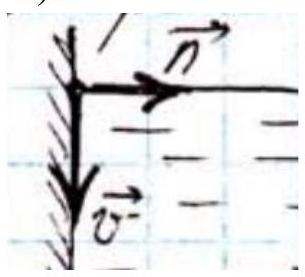
\includegraphics[width=0.2\textwidth]{2023_05_21_6e9b4e8657e82b213c6ag-13}
\end{figure}


a) если стенка неподвижна, то условие непротекания:
$
\left.\vec{v} \cdot \vec{r}\right|_{\text {граница }}=0
$

б) если стенка движется:
$
\left.\vec{v} \cdot \vec{r}\right|_{\text {граница }}=D
$
где D -скорость движения стенки по нормали к ней.

\begin{enumerate}
  \setcounter{enumi}{1}
  \item Граница «жидкость-воздух»
\end{enumerate}

а) если пренебречь атмосферным давлением:
$
\left.\vec{v} \cdot \vec{r}\right|_{\text {граница }}=0
$


б) $\left.\mathrm{p}\right|_{\Gamma}=p_{\text {aтм }}-$ если пренебречь капиллярными эффектами


в) $\left.\mathrm{p}\right|_{\Gamma}-\mathrm{p}_{\text {атм }}=\sigma\left(1 / \mathrm{R}_1-1 / \mathrm{R}_2\right)-$ с учетом капиллярных давлений


\section{Идеальная жидкость. Уравнения Эйлера в форме Громеки- Лэмба. Интеграл Бернулли. Интеграл Коши-Лагранжа. Примеры.}

\textbf{Модель идеальной жидкости} - простейшая модель движущейся жидкости. Не учитывает наличие внутреннего трения (вязкости). По площадкам соприкосновения двух объемов действуют только нормальные к площадкам напряжения, касательных нет.

Модель идеальной жидкости применяется для изучения течения с большими скоростями, кавитационных течений, течений со свободными границами. В рамках данной модели считается, что нет потерь механической энергии.

В идеальной жидкости тензор напряжений имеет вид:

$$
p_{i j}=-p E_{n}=\left(\begin{array}{ccc} 
-p & 0 & 0 \\
0 & -p & 0 \\
0 & 0 & -p
\end{array} \right)
$$

Уравнение движения идеальной жидкости (Уравнение Эйлера):

$$
\rho\left(\frac{\partial \vec{v}}{\partial t}+(\vec{v} \nabla) \vec{v}\right)=-\mathrm{gradp}+\rho \vec{f}
$$

Где $v$ - скорость потока, f-вектор массовой плотности внешних сил.

Если левую часть переписать в виде:

$$
\frac{\partial \vec{v}}{\partial t}+(\vec{v} \nabla) \vec{v}=\frac{\partial \vec{v}}{\partial t}+\mathrm{grad} \frac{v^{2}}{2}+[\mathrm{rot} \vec{v} \times \vec{v}]
$$

Получится \textbf{уравнение Эйлера в форме Громеки-Лэмба:}

$$
\rho\left(\frac{\partial \vec{v}}{\partial t}+\mathrm{grad} \frac{v^{2}}{2}+[\mathrm{rot} \vec{v} \times \vec{v}]\right)=-\mathrm{gradp}+\rho \vec{f}
$$

Данная форма записи позволяет получить вывод интеграла Бернули:

\begin{enumerate}
  \item Считаем жидкость идеальной

  \item Течение стационарно, т.е. $\frac{\partial \mathbf{v}}{\partial t}=0$

  \item Жидкость несжимаема $\rho=$ const

  \item Объемные силы потенциальны, т.е. $\mathbf{F}=\mathrm{grad}(\mathbf{u})$ (u-потенциальное поле энергий)

  \item Будем рассматривать проекции на линии тока, которая совпадает с траекторией

\end{enumerate}


\begin{figure}[h!]
    \centering
    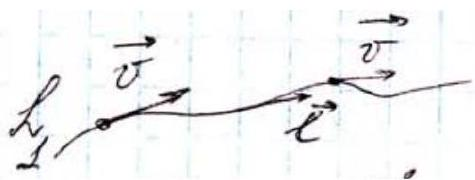
\includegraphics[width=0.5\textwidth]{2023_05_21_6e9b4e8657e82b213c6ag-14(2)}
\end{figure}

Домножим уравнение Эйлера в форме Громеки-Лэмба на $l$ - вектор касательной к линии тока. Тогда:

$$
\begin{gathered}
\rho\left(\mathrm{grad} \frac{v^{2}}{2}+[\mathrm{rot} \vec{v} \times \vec{v}]\right)=-\mathrm{grad} p+\rho \vec{f} \mid \cdot \vec{l} \\
\rho\left(\left(\mathrm{grad} \frac{v^{2}}{2}\right) \cdot \vec{l}+([\mathrm{rot} \vec{v} \times \vec{v}]) \cdot \vec{l}\right)=-\mathrm{grad} p\cdot \vec{l}+\rho \vec{f} \cdot \vec{l} \\
([\mathrm{rot} \vec{v} \times \vec{v}]) \cdot \vec{l})=0 \text { так как векторы ортонормальны } \\
\vec{f}=\mathrm{grad}(u)
\end{gathered}
$$

Получаем уравнение:

$$
\mathrm{grad}\left(\rho \frac{v^{2}}{2}+p-\rho u\right) \cdot \vec{l}=0
$$

$\Gamma$ радиент $=0$, если:

$\rho \frac{v^{2}}{2}+p-\rho u=$ const вдоль линий тока

\textbf{Этот закон называется интегралом Бернулли}


Примеры:


a) Стачионарное течение жидости из сосуда
\begin{figure}[h!]
    \centering
    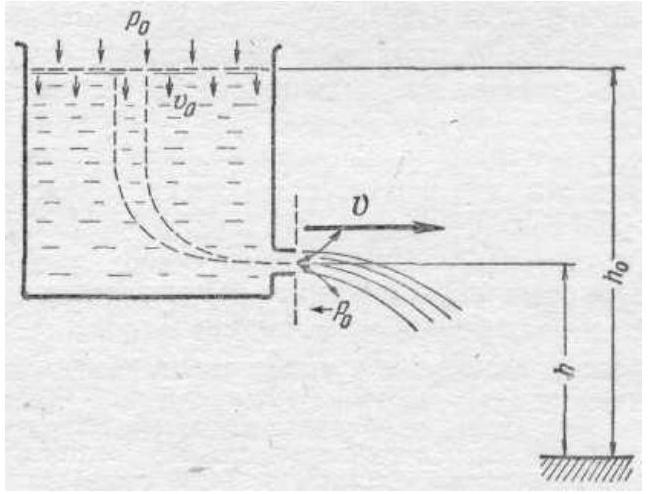
\includegraphics[width=0.5\textwidth]{2023_05_21_6e9b4e8657e82b213c6ag-15}
\end{figure}


Сверху: $\mathrm{p}=\mathrm{p}_{\text {атм }}, \vec{v} \approx 0$ так как сосуд достаточно большой, $\mathrm{z}=\mathrm{h}_{0}$

В дырке на дне: $\mathrm{p}=\mathrm{p}_{\text {атм }}, \mathrm{z}=\mathrm{h}$

Задача состоит в нахождении скорости вытекания воды $\mathrm{v}$

Пусть $\mathrm{H}=\mathrm{h}_{\mathrm{o}}-\mathrm{h}$

Тогда запишем уравнение Бернулли для точки сверху и для точки в дырке на дне (они будут равны, так как уравнение Бернулли должно быть постоянным):

Сверху: $p_{\text {атм }}+\rho g h_{0}$

В дырке: $\rho \frac{v^{2}}{2}+p_{\text {атм }}+\rho g h$

Приравниваем: $\rho \frac{v^{2}}{2}+p_{\text {атм }}+\rho g h=p_{\text {атм }}+\rho g h_{0}$

Тогда: $\rho \frac{v^{2}}{2}=\rho g H$

Выражая скорость из данного уравнения, получаем формулу Торричелли:

$$
v=\sqrt{2 g H}
$$

б) Работа трубки Пито - Прандтля: аэродинамический прибор для измерения динамического давления.

\begin{figure}[h!]
    \centering
    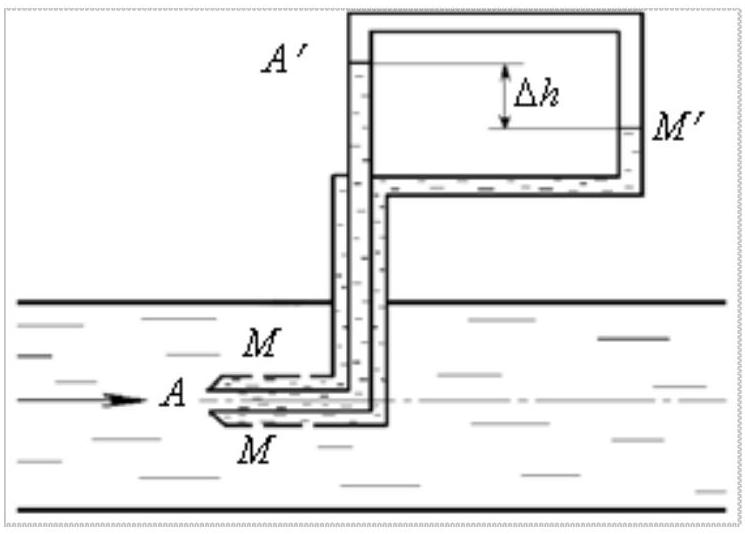
\includegraphics[width=0.5\textwidth]{2023_05_21_6e9b4e8657e82b213c6ag-16(1)}
\end{figure}

Через отверстие А происходит измерение динамического давления. Через отверстия М измеряется статическое давление жидкости.

Записываем уравнение Бернулли для точек А и М:

$$
p_{M}=p_{A}+\rho \frac{v^{2}}{2}
$$

Тогда скорость потока жидкости:

$$
v=\sqrt{\frac{2\left(p_{M}-p_{A}\right)}{\rho}}
$$

Применим для идеальной жидкости в случае потенциальньх течений: $\rho=\mathrm{const}, \vec{v}=\mathrm{grad} \varphi, \vec{f}=$ $\mathrm{grad} \Phi$, где $\Phi$ - потенциал массовых сил, $\phi$ - потенциал скорости. Тогда применим уравнение Эйлера в форме Громеки-Лэмба:
$$
\rho\left(\frac{\partial \vec{v}}{\partial t}+\mathrm{grad} \frac{v^2}{2}+[\mathrm{rot} \vec{v} \times \vec{v}]\right)=-\mathrm{grad} p+\rho \vec{f}
$$
С учетом того, что для потенциального поря rot $=0$, то
$$
\rho\left(\frac{\partial \overrightarrow{\nabla \varphi}}{\partial t}+\mathrm{grad} \frac{(\overrightarrow{\nabla \varphi})^2}{2}+[\mathrm{rot} \vec{v} \times \vec{v}]\right)=-\vec{\nabla} p+\rho \overrightarrow{\nabla \Phi}
$$
Тогда получаем:
$$
\mathrm{grad}\left(\frac{\partial \varphi}{\partial t}+\frac{(\nabla \varphi)^2}{2}+\frac{p}{\rho}-\Phi\right)=0
$$
Градиент будет равен нулю только если выражение в скобках будет константой:
$$
\frac{\partial \varphi}{\partial t}+\frac{(\nabla \varphi)^2}{2}+\frac{p}{\rho}-\Phi=\mathrm{const}
$$
 \textbf{интеграл Коши-Лагранжа}, выполняется во всей жидкости. Константа зависит только от времени.

 
Пример: Жидкость в поле сильы тяжести.

\section{Модель линейно-вязкой несжимаемой жидкости. Уравнения Навье-Стокса. Полная система уравнений. Условие прилипания на границе с твердым телом. Понятие о ламинарном и турбулентном режимах течения.}


В отличие от невязкой идеальной жидкости, в вязкой присутствует внутреннее трение (вязкость), которое приводит к диссипации энергии. Согласно Ньютону: касательные напряжения трения в прямолинейнодвижущейся вязкой жидкости пропорционально изменению скорости по нормали к направлению движения жидкости:
\begin{figure}[h!]
    \centering
    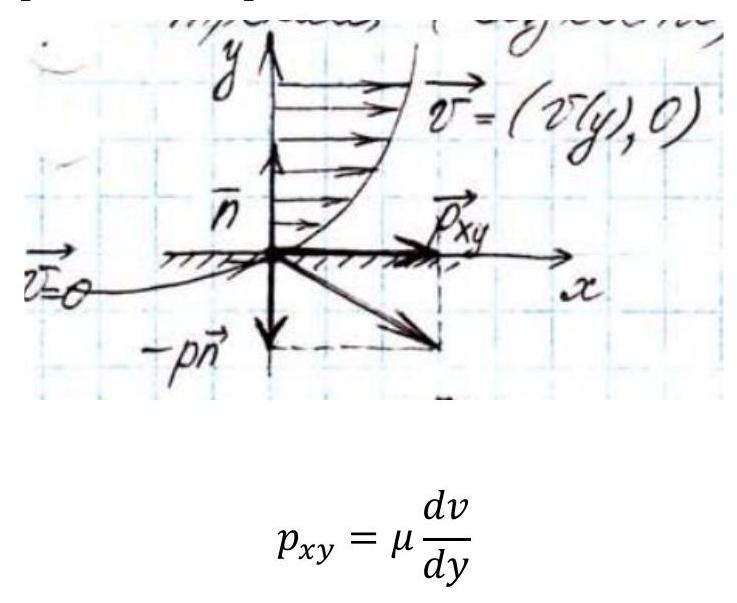
\includegraphics[width=0.5\textwidth]{2023_05_21_6e9b4e8657e82b213c6ag-17}
\end{figure}
где $\mu-$ коэффициент вязкости

В вязкой жидкости тензор напряжений имеет вид: $\boldsymbol{p}_{i j}=-p \delta_{i j}+\tau_{i j}$, где $\boldsymbol{\delta}_{i j}-$ символ Кронекера, $\tau_{i j}-$ тензор вязких напряжений. В несжимаемой жидкости: $\tau_{i j}=2 \mu e_{i j}$

\textbf{Закон Навье-Стокса для несжимаемой жидкости:}
$$
\begin{aligned}
& p_{i j}=-p \delta_{i j}+2 \mu e_{i j} \\
& e_{i j}=\frac{1}{2}\left(\frac{\partial v_{i}}{\partial x_{j}}+\frac{\partial v_{j}}{\partial x_{i}}\right)
\end{aligned}
$$

Тогда тензор напряжений можно записать:

$$
\left(p_{i j}\right)=\left(\begin{array}{cc}
-p & 0 \\
0 & -p
\end{array}\right)+\left(\begin{array}{cc}
0 & \mu \frac{d v}{d y} \\
\mu \frac{d v}{d y} & 0
\end{array}\right)=\left(\begin{array}{cc}
-p & \mu \frac{d v}{d y} \\
\mu \frac{d v}{d y} & -p
\end{array}\right)
$$

\begin{enumerate}
  \item Закон сохранения массы для несжимаемой жидкости: $\mathrm{div} v=0$
  \item Уравнение движения жидкости (уравнение Эйлера):
\end{enumerate}

$$
\rho\left(\frac{\partial \vec{v}}{\partial t}+(\vec{v} \nabla) \vec{v}\right)=-\mathrm{gradp}+\rho \vec{f}
$$

Где тензор напряжений

$$
p_{i j}=-p \delta_{i j}+2 \mu e_{i j}=-p \delta_{i j}+\mu \mathrm{grad} vec{v}
$$

Тогда уравнение движения примет вид (\textbf{это уравнение Навье-Стокса}):

$$
\rho\left(\frac{\partial \vec{v}}{\partial t}+(\vec{v} \nabla) \vec{v}\right)=-\mathrm{grad} p+\mu \Delta \vec{v}+\rho \vec{f}
$$

Где $\Delta$ - оператор Лапласа.


Система уравнений 1 и 2 с заданными граничными условиями - полная система уравнений.

\textbf{Граничные условия:}


a) Жидкость-твердое (стенка):
$\left.\mathbf{v}\right|_{\Gamma}=\mathbf{D}-$ где $\mathrm{D}$ скорость стенки

(В частном случае, для неподвижной стенки $\left.\mathbf{v}\right|_{\Gamma}=\mathbf{0}$ - \textbf{условие прилипания})

б) Граница между двумя вязкими жидкостями:

\begin{enumerate}
  \item $\left.\mathbf{v}_2\right|_{\Gamma}=\left.\mathbf{v}_1\right|_{\Gamma}-$ равенство скоростей

  \item $\left.\left(\mathrm{p}^{1}{ }_{\mathrm{ij}}-\mathrm{p}^{2} _\mathrm{ij}\right)\right|_{г} \mathrm{n}_{\mathrm{j}}=0$ равенство действующих друг на друга сил

\end{enumerate}

\textbf{Ламинарное и турбулентное движение жидкости:}

\begin{figure}[h!]
    \centering
    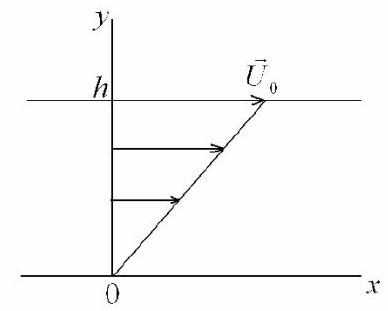
\includegraphics[width=0.5\textwidth]{2023_05_21_6e9b4e8657e82b213c6ag-18}
\end{figure}


Ламинарное движение - плоскопараллельное, когда линии тока - прямые линии. Это выполняется когда скорость направлена только по оси $\mathrm{x}$, а составляющая по у $\mathrm{V}_{\mathrm{y}}=0$.

Пример - движение жидкости между параллельными неподвижными пластинами:
\begin{figure}[h!]
    \centering
    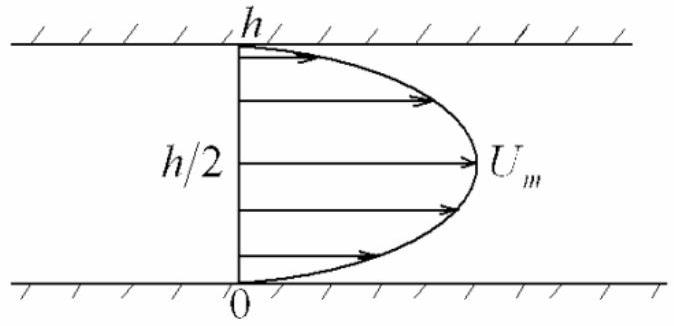
\includegraphics[width=0.5\textwidth]{2023_05_21_6e9b4e8657e82b213c6ag-18(1)}
\end{figure}

Турбулентное - возмущенное, неустойчивое течение жидкости. Характеристикой, которая разграничивает эти режимы течения, является число Рейнольдса.

\textbf{Число Рейнольдса} - безразмерная величина, характеризующая отношение силы инерции к силе трения:

$$
R e=\frac{\rho v^{2}}{l}: \frac{\mu v}{l^{2}}=\frac{\rho v l}{\mu}
$$

Где v - средняя скорость движения (характерная скорость), l - характерная длина (размер тела или ширина канала), $\rho$ - плотность жидкости. $\mu$ - вязкость.

При $\mathrm{Re}<\mathrm{Re}_{\text {кр }}$ наблюдается упорядоченное ламинарное течение.

При $\mathrm{Re}>\mathrm{Re}_{\text {кр }}-$ течение турбулентное, хаотическое.

\section{Определяюшие параметры явления. Класс систем единиц. Размерность физической величины. П-теорема теории размерностей. Моделирование физических процессов на основе П-теоремы. Критерии подобия. Примеры (число Рейнольдса).}
\textbf{Физические величины:}
\begin{enumerate}
  \item Первичные (основные) величины: L - единица длины; $\mathrm{M}$ - единица массы; $\mathrm{T}$ единица времени. Образуют класс $\{\mathrm{LMT}\}$. Пример: международная система СИ и СГС.

  \item Вторичные (производные) величины: $\rho, \mathrm{v}, \mathrm{F}$ и тд

\end{enumerate}

Цель физического исследования --- поиск связи между численными значениями искомого параметра а и численными значениями других параметров $a_{1}, a_{2}, a_{3} \ldots a_{n}$ от которых он зависит. а --- определяемый параметр. $\mathrm{a}_{1}, \mathrm{a}_{2}, \mathrm{a}_{3} \ldots \mathrm{a}_{\mathrm{n}}$ - определяющие параметры.

$$
a=f\left(a_{1}, a_{2}, a_{3} \ldots a_{n}\right)
$$

Пусть определяемый и определяющие параметры измеряются в системе LMT. Тогда размерность каждой величины представляется в виде:

$$
\begin{gathered}
\mathrm{dim} a=[a]=L^{\alpha} M^{\beta} T^{\gamma} \\
\mathrm{dim} a_{i}=\left[a_{i}\right]=L^{\alpha i} M^{\beta i} T^{\gamma i}
\end{gathered}
$$

Если $\alpha, \beta, \gamma=0$ то такая физическая величина безразмерна.

\underline{Определение 1.} Параметры $\mathrm{a}_{1}, \mathrm{a}_{2}, \mathrm{a}_{3} \ldots \mathrm{a}_{\mathrm{n}}$ размерно независимыь, если из них можно составитьтолько тривиальную безразмерную комбинацию, т.е.:

$$
\left[\mathrm{a}_{1}{ }^{\mathrm{k}_1} \mathrm{a}_{2}{ }^{\mathrm{k}_2} \mathrm{a}_{3}{ }^{\mathrm{k}_3} \ldots \mathrm{a}_{\mathrm{n}}^{\mathrm{k_n}}\right]=1 \text {, если для всех } \mathrm{ki}=0 \text {, для любых } \mathrm{i}
$$

Пример: $\mathrm{v}- \text{м/c}, \rho-\text{кг/м3} $ --- размерно независимы

$\mathrm{v}-\text{м/c}, \quad \rho-\text{кг/м3}, \quad\mathrm{l}-\text{м},\quad \mu-\text{кг/(м*с)}$ размерно зависимы: из них можно составить безразмерную величину - число Рейнольдса.

(\textbf{Число Рейнольдса} - безразмерная величина, характеризующая отношение силы инерции к силе трения:
$
R e=\frac{\rho v^{2}}{l}: \frac{\mu v}{l^{2}}=\frac{\rho v l}{\mu}
$)


\underline{Определение 2.} Размерно независимые параметры $\mathrm{a}_{1}, \mathrm{a}_{2}, \mathrm{a}_{3} \ldots \mathrm{a}_{\mathrm{k}}$ из системы параметров а $\mathrm{a}_{1}, \mathrm{a}_{2}, \mathrm{a}_{3}$ ... $a_{\mathrm{n}}(\mathrm{k}\leq\mathrm{n})$ образуют максимально размерно независимую подсистему параметров, если $\mathrm{k}=\mathrm{n}$ или любая подсистема $\mathrm{k}+1$ параметров будет размерно зависимой.

\textit{П-теорема:}
\begin{enumerate}
  \item Есть некоторый класс систем единиц

  \item Есть определяемый параметр а и определяющие параметры $a_{1}, a_{2}, a_{3} \ldots a_{n}$; все параметры измеряются в данном классе; между параметрами существует следующее физическое соотношение:

\end{enumerate}

$$
a=f\left(a_{1}, a_{2}, a_{3} \ldots . a_{n}\right)
$$

\begin{enumerate}
  \setcounter{enumi}{2}
  \item Вид функции $\mathrm{f}$ не меняется при изменении масштабов в классе

  \item $\mathrm{a}_{1}, \mathrm{a}_{2}, \mathrm{a}_{3} \ldots \mathrm{a}_{\mathrm{k}}$ - максимально размерно независимая подсистема параметров

\end{enumerate}

Тогда:
Размерность определяемого параметра а выражается через размерности параметров $\mathrm{a}_{1}, \mathrm{a}_{2}$, a3 $\ldots \mathrm{a}_{\mathrm{k}}$, а соотношение между $\mathrm{n}+1$ размерной величиной можно записать в виде соотношения между $\mathrm{n}+1-k$ безразмерными величинами:

$$\begin{aligned}  
&\Pi=\varphi\left(\Pi_{1}, \Pi_{2}, \ldots \Pi_{n-k}\right)\\
&\Pi=\mathrm{a} /\left(\mathrm{a}_{1}{ }^{\mathrm{m} 1} \mathrm{a}_{2}{ }^{\mathrm{m} 2} \mathrm{a}_{3}{ }^{\mathrm{m} 3} \ldots \mathrm{a}_{\mathrm{k}}{ }^{\mathrm{mk}}\right) ; \\
&\Pi_{1}=\mathrm{a}_{\mathrm{k}+1} /\left(\mathrm{a}_{1}{ }^{\mathrm{p} 1} \mathrm{a}_{2}{ }^{\mathrm{p}^{2}} \mathrm{a}_{3}{ }^{\mathrm{p} 3} \ldots a_{k}{ }^{\mathrm{pk}}\right) ; \\
&\Pi_{n-k}=a_{k+1} /\left(a_{1}{ }^{q^{1}} \mathrm{a}_{2}{ }^{\mathrm{q} 2} \mathrm{a}_{3}{ }^{\mathrm{q} 3} \ldots a_{k}{ }^{\mathrm{qk}}\right)
\end{aligned}
$$

\textbf{Подобие физических явлений}
Одно из важных применений П-теоремы теория подобия. Очень часто нужно установить значения величины $\mathrm{a}^{\mathrm{H}}$ натурального объекта по измеренной на модели величине $\mathrm{a}^{\mathrm{M}}$. Если для величин $\mathrm{a}_{1}{ }^{\mathrm{M}}, \mathrm{a}_{2}{ }^{\mathrm{M}}, \ldots \mathrm{a}_{3}{ }^{\mathrm{M}}$ и $\mathrm{a}_{1}{ }^{\mathrm{H}}, \mathrm{a}_{2}{ }^{\mathrm{H}}, \ldots \mathrm{a}_{3}{ }^{\mathrm{H}}$ совпадают соответствующие эти значениям безразличные числа $\Pi_{1}, \ldots . \Pi_{n-k}$. То пользуясь Пи-теоремой находим $\mathrm{a}^{\mathrm{H}}$ :

$$
a^{\mathrm{H}}=a^{\mathrm{M}}\left(\frac{\mathrm{a}_{1}^{\mathrm{H}}}{\mathrm{a}_{1}^{\mathrm{M}}}\right) \cdot\left(\frac{\mathrm{a}_{2}^{\mathrm{H}}}{\mathrm{a}_{2}^{\mathrm{M}}}\right) \cdots\left(\frac{a_{l}^{\mathrm{H}}}{\mathrm{a}_{l}^{\mathrm{M}}}\right)
$$

Безразмерные числа $\Pi_{1}, \ldots \Pi_{\mathrm{n}-\mathrm{k}}$ называют критериями подобия. Два явления одной физической природы называются подобными, если их критерии подобия соответственно одинаковы.

Примерами таких критериев подобия в гидродинамике могут является числа

Рейнольдса и Фруда (соотношение между силой инерции и внешней силой $\mathrm{Fr}=\mathrm{v}^{2} / \mathrm{gL}$ ).

Так, чтобы добиться одинаковых чисел Рейнольдса,вязкость жидкости, обтекающей модель, должна быть в 1000 раз меньше вязкости воды. Поскольку такие условия создать невозможно, силу трения приходится рассчитывать по эмпирическим формула.

Число Рейнольдса --- безразмерная величина характеризующая отношение силы инерции к силе трения:

$$
R e=\frac{\rho v^{2}}{l}: \frac{\mu v}{l^{2}}=\frac{\rho v l}{\mu}
$$

Где v - характерная скорость (скорость движения тела, средняя скорость в сечении канала) $l$ - характерная длина(размер тела или ширина канала). $\rho$ - плотность жидкости. $\mu$ - вязкость. При $\mathrm{Re}<\mathrm{Re}_{\text {кр }}$ наблюдается упорядоченное ламинарное течение. При $\mathrm{Re}>\mathrm{Re}_{\text {кр }}-$ течение турбулентное, хаотическое.

Другие примеры критериев подобия:

\begin{enumerate}
  \item При изучении упругих деформаций конструкции под воздействием внешних сил основным является  коэффициент Пуассона (величина отношения относительного поперечного сжатия к относительному продольному растяжению)

  \item Для механического движения получается из уравнения, выражающего второй закон Ньютона и называется числом Ньютона:

\end{enumerate}

$$
N e=\frac{F t^{2}}{m l}
$$
